

With the goal of comparing optimization methods and finding the regime of hyper parameters where multi-region demixing is beneficial, we start with a series of experiment on controlled data where the latent factors are known and used as a ground truth. We first describe how the dataset was created and then characterize how performance depends on the number of samples and the number of latent factors (cell types).


\subsubsection*{Creating the mixture dataset}
We created controlled mixtures from a set of real transcriptome measurements, collected from isolated cells



We gathered profiles for the 3 population of cell types in the brain: neurons, astrocytes and oligodendrocytes. Each profile is represented by 14580 genes. The cell type profiles were extracted from 7 brain regions:  cortex layer 5A, cortex layer 5B, cortex layer 6, striatum, cerebellum, brainstem and the spinal cord \cite{okaty2011cell}. For each region, we mixed the profiles using ratio taken from the literature \cite{Herculano2014}. cortical regions ( 0.7; 0.1;0.2) , cerebellum (0.5; 0.15; 0.35) , other (0.65;  0.1;0.25)  (neuron, astrocytes, oligodendrocytes).

We have added variability to the proportions of the samples by multiplying them by random value [0,1] and scaling back so that they sum to 1.
Finally, we introduced noise for each sample by multiplying it with by a normal random variable with unit mean. We insure that the normally distributed number is positive.

We evaluated the reconstructed profiles by computing their spearman correlation with the true profiles. We then, matched the best true profiles to the reconstructed profiles.

Each time we sampled n noisy samples and reconstructed the profiles using these samples. The error bars in figure  represented the sem over 30 repetitions.  

{\bf{Move to the experiments section? Also fix the 1st sentence}} Since NMF is a non-convex problem bench-marked a couple of methods on our problem. We wanted to test if when initialized using the same starting points they will perform differently. We tested 4 optimization techniques and found that all performed better with more samples. When the number of sample is sufficiently large we did not observe much difference in the performance of the different methods. while in a small number of samples the block-pivoting and the active-set performed slightly better (both had the same level of performance) Figure \ref{fig:controlled_exp}.

\subsubsection*{analyzing number of samples}
We notice that in the regime of limited samples there is sweet spot where we benefit from using regularization over the naive cases. As we increase the number of samples the benefit that we gain by using our method diminishes Figure \label{fig:controlled_exp}(b). With enough samples we solving the individual problems performs almost just as well. 



\begin{figure}[!hbt]
   (a) \hspace{120pt}(b) \hspace{120pt}(c) \hspace{120pt}
   \centering
     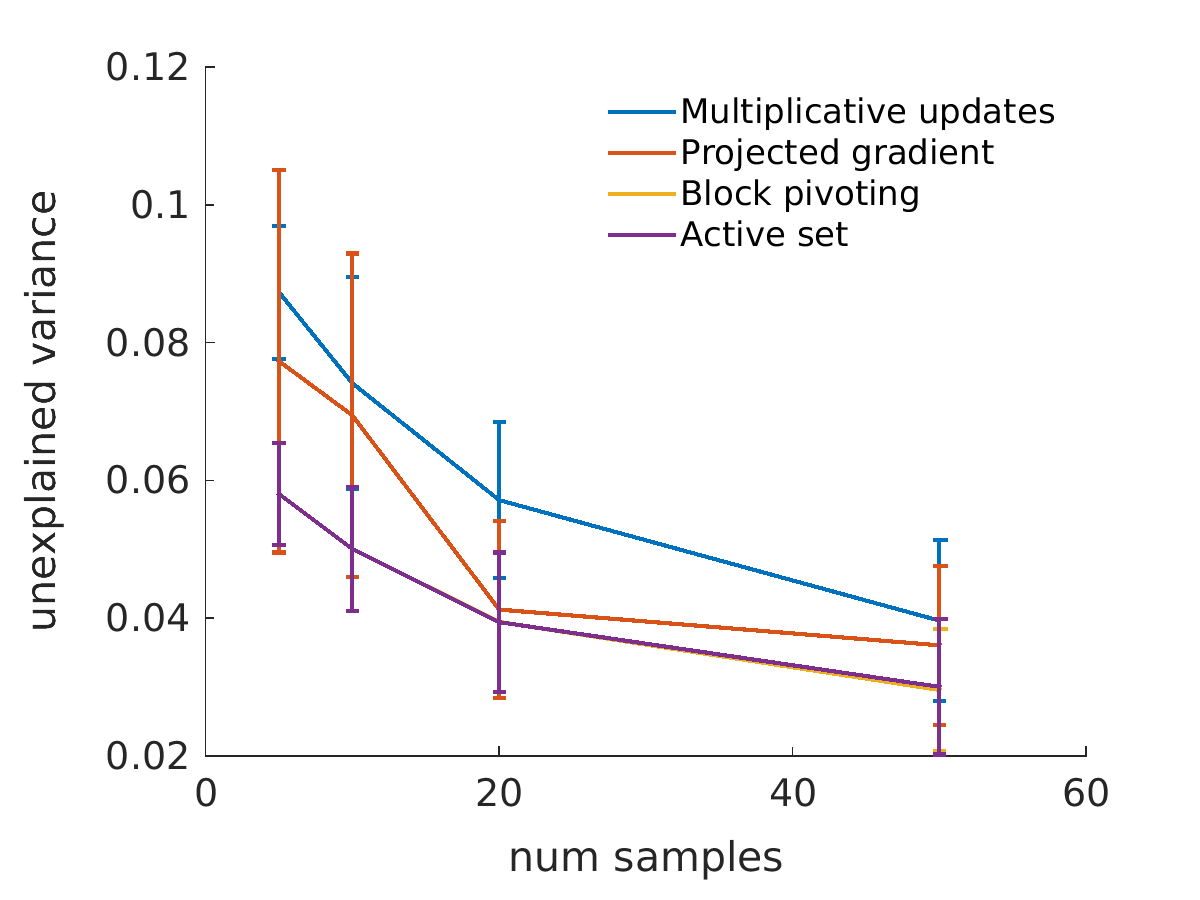
\includegraphics[width=0.32\textwidth]{methods}
     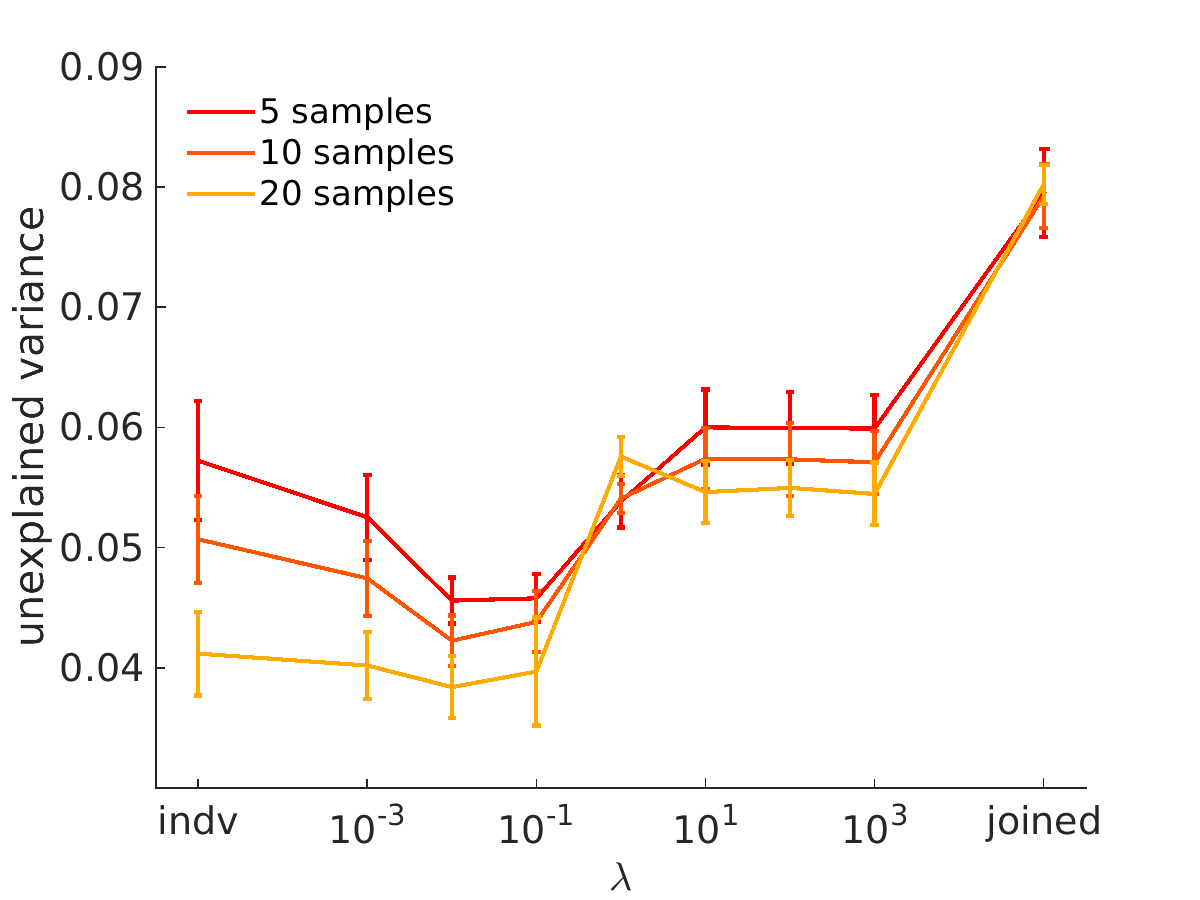
\includegraphics[width=0.32\textwidth]{lambda_sample_with20}
     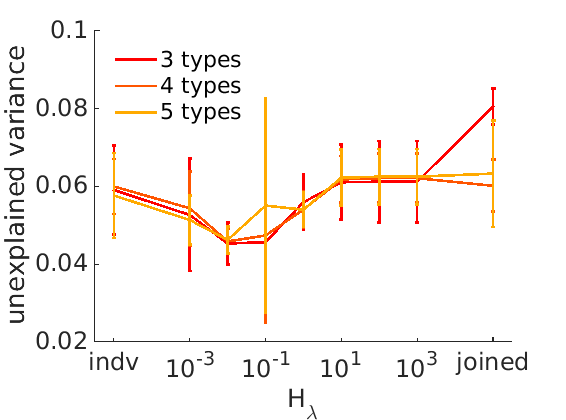
\includegraphics[width=0.32\textwidth]{num_types}
    \caption{The effect of $\lambda$ on reconstruction}, 
    (a)  With a single region, all optimization method perform better as we introduced more samples. With a limited number of samples the active set and the block pivoting approaches performed the best. (b) Using multiple regions, the regularized connection between the region profiles help to reconstruct the original profiles. This is especially noticeable when only few samples are available for each region. (c) ????
    \label{fig:controlled_exp}
\end{figure}




\subsubsection*{analyzing number of cell types}

As we increase the number of types the we are able to numerically better reconstruct the data matrix because we are allowing an approximation with of a larger rank. The reconstructed was able to recover the original profiles and to provide other vectors. Overall it seems that this coincide with Ockham's razor and we can select simplest model which still capture the data. 



